\documentclass{article}
% translate with >> pdflatex -shell-escape <file>

% This file is used as unit test for pgfplots, copyright by Christian Feuersaenger.
% 
% See
%   http://pgfplots.sourceforge.net/pgfplots.pdf
% for pgfplots.
%
% Any required input files (for <plot table> or <plot file> or the table package) can be downloaded
% at
% http://www.ctan.org/tex-archive/graphics/pgf/contrib/pgfplots/doc/latex/
% and
% http://www.ctan.org/tex-archive/graphics/pgf/contrib/pgfplots/doc/latex/plotdata/

\usepackage{pgfplots}
\pgfplotsset{compat=newest}

\pagestyle{empty}

\begin{document}

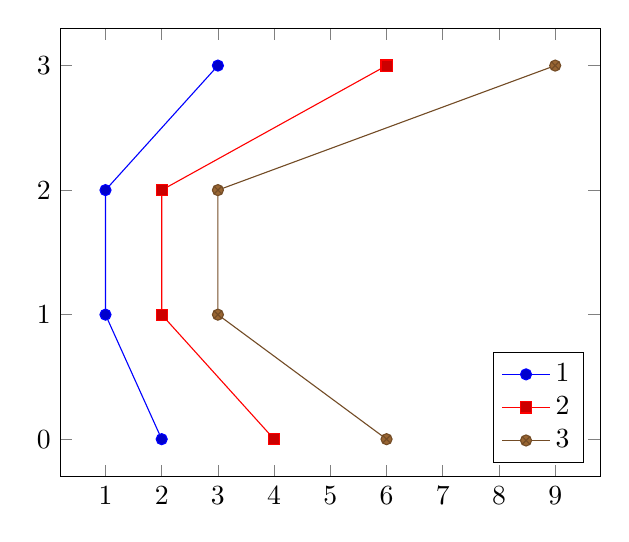
\begin{tikzpicture}
%\tracingmacros=2\tracingcommands=2
	\begin{axis}[stack plots=x,
		legend style={at={(0.97,0.03)},anchor=south east},
		xtick={0,...,30},
	]
	\addplot coordinates {(2,0) (1,1) (1,2) (3,3)};
	\addplot coordinates {(2,0) (1,1) (1,2) (3,3)};
	\addplot coordinates {(2,0) (1,1) (1,2) (3,3)};
	\legend{1,2,3}%
	\end{axis}
%\tracingmacros=0\tracingcommands=0
\end{tikzpicture}
\end{document}
